\documentclass[a4paper]{article}
\usepackage[margin=3cm]{geometry}
\usepackage{graphicx} % Required for inserting images
\usepackage{float}
\usepackage{multicol}

\title{Exploratory Data Analysis - report}
\author{github.com/Macsok}
\date{October 2024}

\begin{document}

\begin{titlepage}
   \begin{center}
        \vspace*{4cm}

        \Huge
        \textbf{Exploratory Data Analysis}
        \vspace{0.5cm}

        \LARGE
        Data Investigation Report
        \vspace{2.5cm}
       
        \textbf{github.com/Macsok}

        \Large
        \vfill
        October 2024   
   \end{center}
\end{titlepage}



% \maketitle

\newpage
\tableofcontents
\newpage

\section{Introduction}
\subsection{What is EDA?}
EDA stands for Exploratory Data Analysis. It’s a crucial step in the data analysis process where you summarize the main characteristics of a dataset, often using visual methods. Here’s the gist:
    \begin{itemize}
        \item Purpose: Understand the data better before jumping into modeling. It helps in uncovering patterns, spotting anomalies, testing hypotheses, and checking assumptions.

        \item Tools and Techniques: Descriptive statistics (mean, median, mode, standard deviation), visualizations (histograms, scatter plots, box plots), and data wrangling (handling missing values, scaling).

        \item Outcome: You get insights that guide your next steps in the data science workflow.
    \end{itemize}
You can think of it as getting to know your dataset inside out, making sure you’re fully prepped before the heavy lifting begins.

\subsection{An aim}
This analysis aims to understand the dataset of 134 cocktails. It aims to identify main characteristics of the cocktails, understand relations between ingredients and distinguish potential groups of similar drinks.

\subsection{An approach}
The approach is based on uncovering pure properties, relations and information from every datum that TheCocktailDB provides us with. It all started by subtle looking and each column and examining its content. The goal was to extrude as much information as we could (even exploring 'createdAt' and 'updatedAt' columns). After testing and making brief reconnaissance we moved to analysing cocktails alone, then ingredients dataframe, next we tried to merged them together and unravel relations between them, finally we analised whole set using scikit-learn library. In other words we started with data type manipulation and clearing data, moved through exploring single properties, and landed on clustering our set and suggesting similar drinks. \textbf{I highly suggest you to go file by file and follow thinking pattern that took us there.}

\subsubsection{Brief overlook of the dataset}
Main part of the data collection consists of \textbf{134} rows and \textbf{11} columns. Here is brief look at it:

\begin{figure}[H]
    \centering
    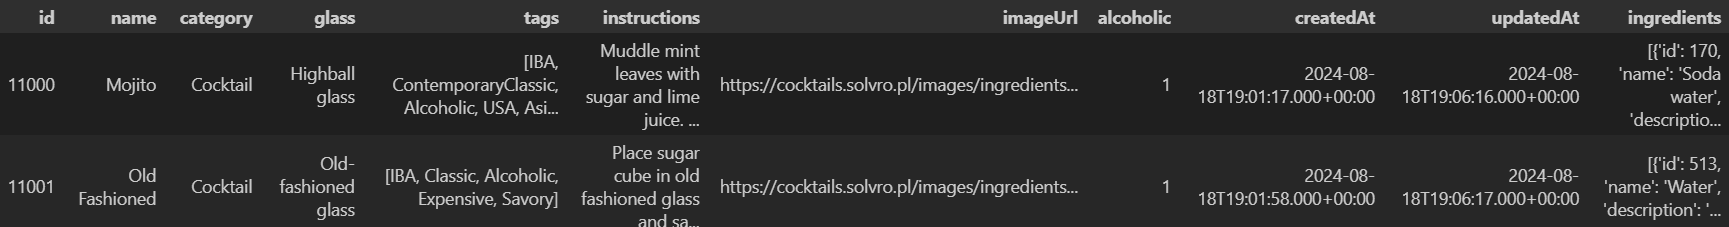
\includegraphics[width=1\linewidth]{base_head.png}
    \caption{TheCocktailDB head}
    \label{fig:TheCocktailDB_head}
\end{figure}

The columns are: id, name, category, glass, tags, instructions, imageUrl, alcoholic, createdAt, updatedAt, ingredients. Every column excpet 'id' and 'alcoholic' have object type. Other two are represented as int64.

In 'ingredients' column there is nested information about ingredients. Each drink have own piece of ingredients information there. If you unpack such block of information there will be data about ingredients needed to prepare such drink. Every record in 'ingredients' table has \textbf{10} attributes. They are as follows: id, name, alcohol, type, percentage, imageUrl, createdAt, updatedAt, measure. After unpacking ingredients data from every cocktail there will be \textbf{531} unique records in the 'ingredients' table.

\begin{figure}[H]
    \centering
    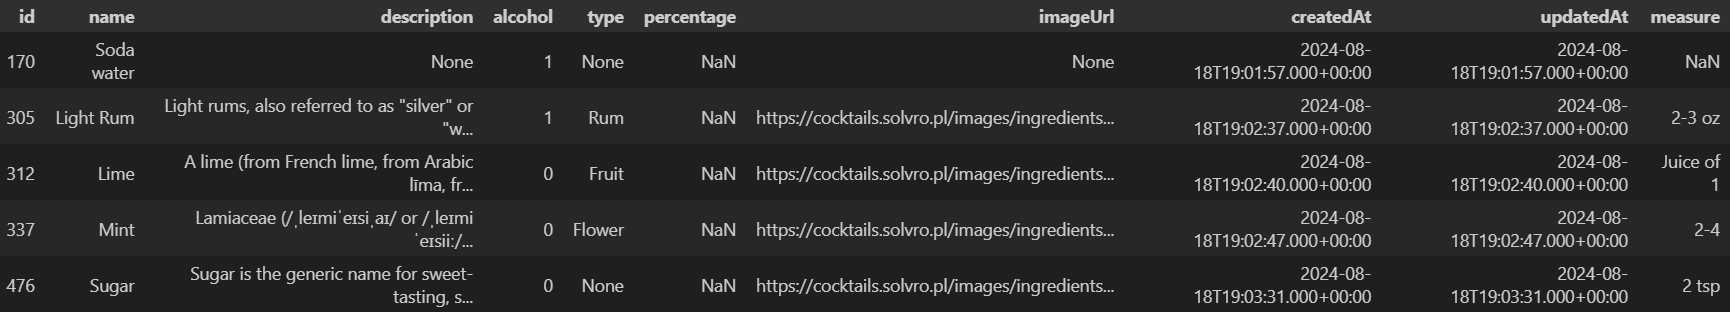
\includegraphics[width=1\linewidth]{ingredients_head.png}
    \caption{A snippet of the 'ingredients' table}
    \label{fig:ingredients_head}
\end{figure}

\section{Data review}
\subsection{Data loading}
In this section, we will demonstrate the steps required to load the dataset into our analysis environment. As we found out data is stored in .json format, so loading it into pandas DataFrame looks like this:
\begin{figure}[H]
    \centering
    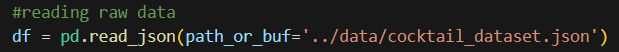
\includegraphics[width=1\linewidth]{loading.png}
    \caption{Loading data and storing it as pandas DataFrame}
    \label{fig:enter-label}
\end{figure}

\subsection{Missing values}
In this section we will examine missing values in our DataFrame and correct type of data in time columns. Figure 4 represents summed rows of missing values in each column of the dataset. We can see that most of the 'tags' column is missing (\textbf{99 out of 134}). Figure 5 shows code used to correct data type in 'createdAt' and 'updatedAt' columns.
\vspace{2cm}

\begin{multicols}{2}

\begin{figure}[H]
    \centering
    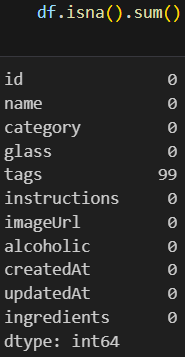
\includegraphics[width=0.4\linewidth]{types.png}
    \caption{Sums on missing values}
    \label{fig:enter-label}
\end{figure}

\columnbreak

\begin{figure}[H]
    \centering
    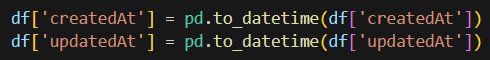
\includegraphics[width=1\linewidth]{type correction.png}
    \caption{Data type correction}
    \label{fig:enter-label}
\end{figure}

\end{multicols}

\subsection{Brief exploration}
After short reconnaissance of the data in our DataFrame you can spot some important properties:
\begin{itemize}
    \item every cocktail is alcoholic
    \item imageUrl won't be useful in the data analysis (at least for us)
    \item id's aren't consistent
    \item 'ingredients' column is stuffed with a .json data
\end{itemize}
In that case further explorations of the dataset will exclude 'imageUrl' and 'alcoholic' columns.

\section{Exploring cocktails alone}
In this section we pay attention only to cocktails - we won't unpack data from 'ingredients' column. In this case we drop four columns: 'ingredients', 'imageUrl', 'alcoholic', 'tags'.
\subsection{Is there something hidden in those times?}
Creating and updating times may seem harmless and boring but is there something hidden? Let's plot them and find out! Figure 6 shows the result, seems that nothing interesting was hidden there. 

\begin{figure}[H]
    \centering
    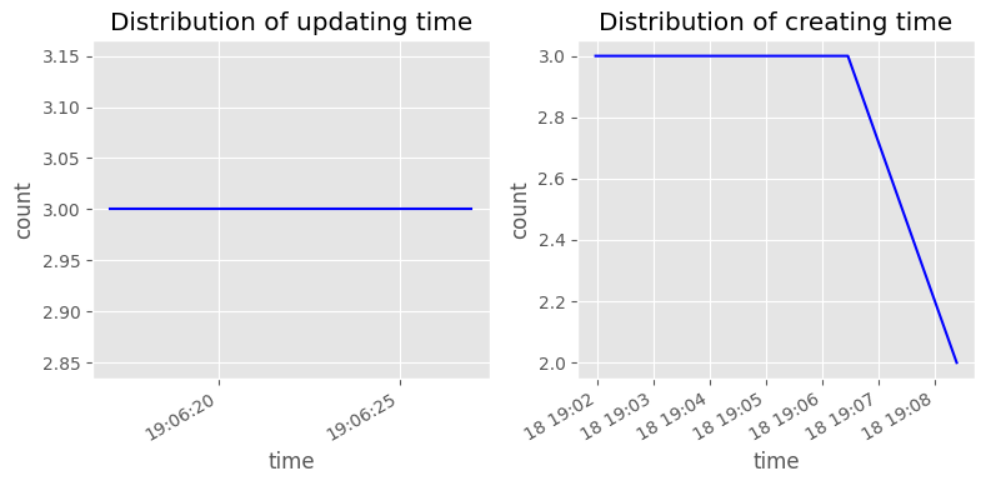
\includegraphics[width=0.8\linewidth]{times cocktails.png}
    \caption{Times of creating and upgrading cocktails}
    \label{fig:enter-label}
\end{figure}

\subsection{Exploring other properties}
Next we will simplify a little and assume that length of the instruction is somehow relevant to level of preparation complexity. We will replace textual value of instructions with the length of it. Below (on Figure 7) you can see brief code and the results of such operation. In this case we can, for example, find relations between type of the glass and the instruction length. Figure 8 presents lenghts of the instruction per every type of glass. Each red dot represents one cocktail. We can spot that Highball glasses tend to have a little longer instructions than Cocktail glasses. Old-fashioned glass drinks' instruction length vary more than Cocktails glass ones which are more regular.

\begin{figure}[H]
    \centering
    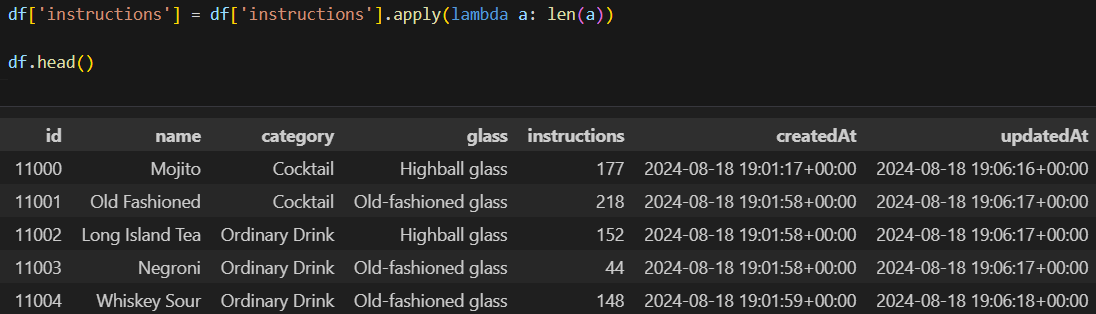
\includegraphics[width=1\linewidth]{simplify.png}
    \caption{Replacement of the instruction and  current look at head of our cocktails data}
    \label{fig:enter-label}
\end{figure}

\begin{figure}[H]
    \centering
    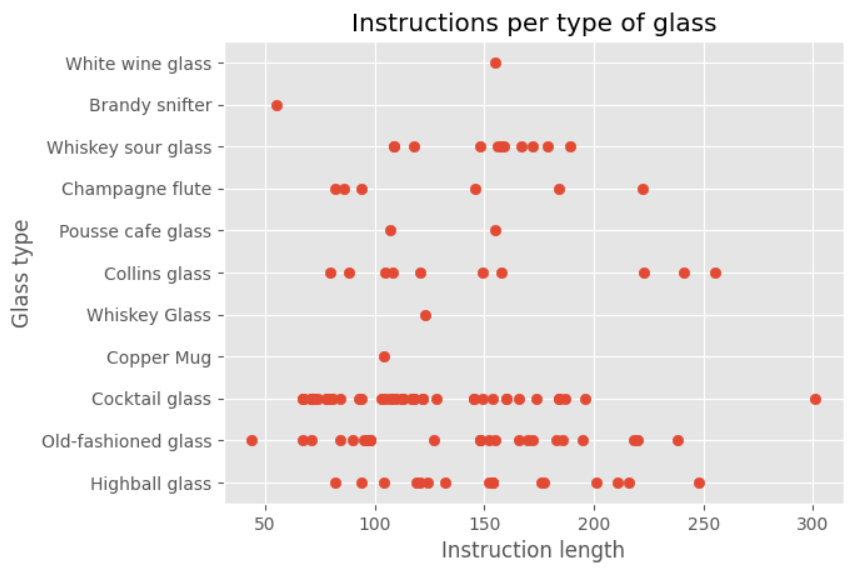
\includegraphics[width=0.8\linewidth]{ins length.png}
    \caption{Length of the instruction per type of the glass}
    \label{fig:enter-label}
\end{figure}

\subsection{Dividing into groups}
Let's take a look at popularity of each drink category. There are three such categories: Punch / Party Drink, Cocktail, Ordinary Drink. To count how many drinks are in each category we will use function: value\_counts(), then we will simply plot it as horizontal bar plot. Here is the result (Figure 9):

\begin{figure}[H]
    \centering
    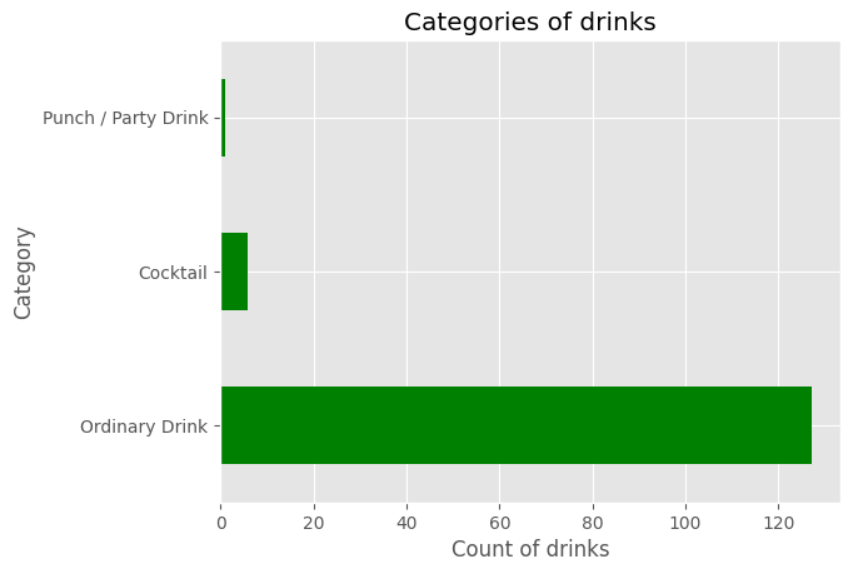
\includegraphics[width=0.7\linewidth]{categories.png}
    \caption{Count of drinks in each category}
    \label{fig:enter-label}
\end{figure}

Similarly we can count the frequency of using each glass type in drinks and present the mon bar plot. This time we will focus on top 10 used glass types.

\begin{figure}[H]
    \centering
    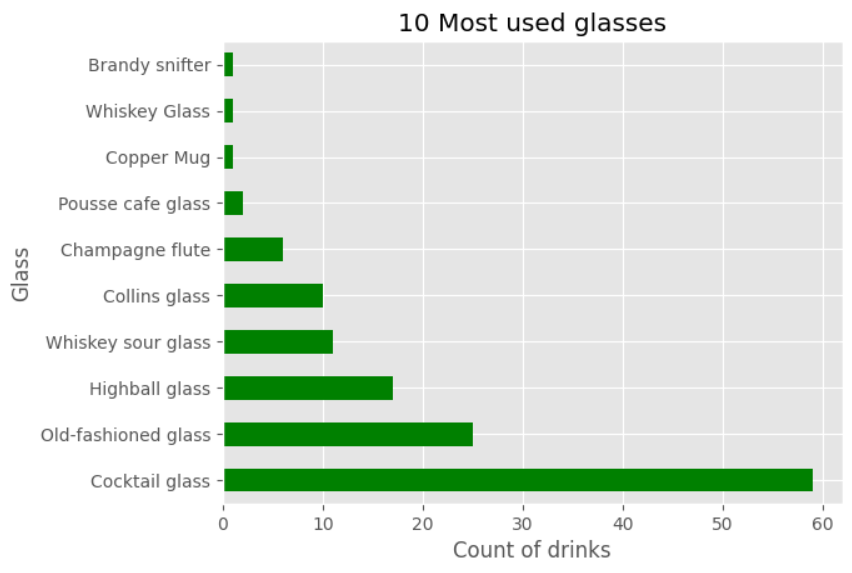
\includegraphics[width=0.9\linewidth]{glass types.png}
    \caption{Top 10 used glasses}
    \label{fig:enter-label}
\end{figure}

As we can see the most commonly used glass type is Cocktail glass, second one is Old-fashioned glass and on third position there is Highball glass. The top one leaves opponents far behind.

\section{Exploring ingredients alone}
In this section we will take closer look on data containing only ingredients of the cocktails. Similarly to the previous section we won't pay attention to the connections between drinks and their ingredients - at least not yet. In this part data about every cocktail ingredients is stored in separate table.

\begin{figure}[H]
    \centering
    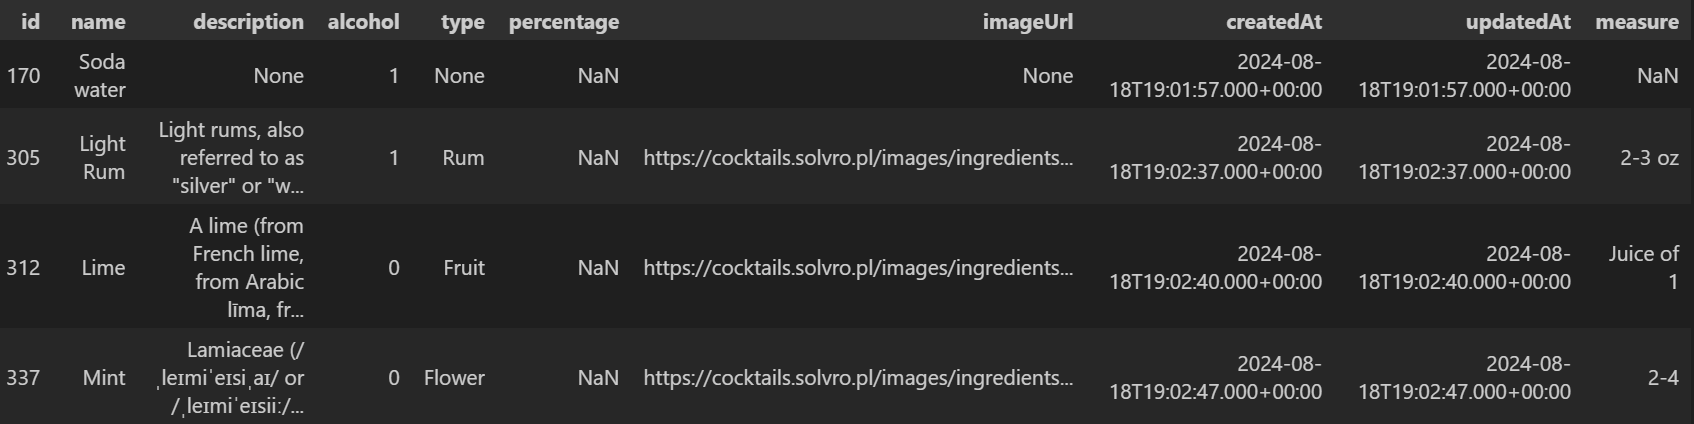
\includegraphics[width=1\linewidth]{ingrhead.png}
    \caption{Head of the ingredients dataframe}
    \label{fig:enter-label}
\end{figure}

\subsection{Missing values and duplicates}
Checking each column shows that many of them have missing values:
\begin{itemize}
    \item 431 records from 'percentage'
    \item 224 records from 'description'
    \item 121 records from 'type'
    \item 35 records from 'measure'
\end{itemize}
Note that a shape of ingredients dataframe is \textbf{11 x 531}.

Each column have it individual explanation of shortage. 'percentage' column is missing values in every record that has 0 percent. To repair this issue we can simply map every NaN value to zero. 'description' column is missing information for simple ingredients such as water. 'type' and 'measure' are just not specified in some cases of the ingredients (missing measure of added water, water and sugar have none type). Due to lack of the information in the 'description' column and not normalized data in 'measure' column we won't consider those in further analysis (normalising measure column could be a fun thing to do...).

There are many duplicates in the 'name' column cause of the usage of similar ingredients in different drinks. For example there are many records of 'Gin' with various types of the measurement.

\subsection{Exploring ingredients}
Before diving into world of relations and connections we can make some corrections in data types of our set. As before we will updated data type in columns which store date information. Furthermore we will map every missing value to 0 (not recommended in every case).

Having prepared data we can start playing with it. Again we will try to extract information from every bit of the data - we will analyze updatig times again (Figure 13). This time it looks more promising as it is not a straight boring line. Most of the updates were made at the beginning - around 19.01 - then it lapsed down and there was another peak of updates around 19.02.30. After it, it went down again. Was there something useful? Well... Maybe not but again - we are here to learn and try to find hidden relations.

\begin{figure}[H]
    \centering
    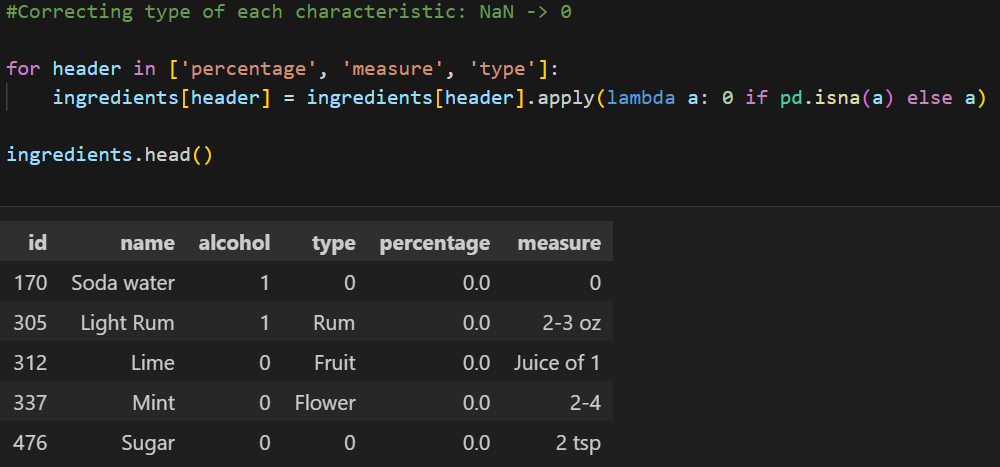
\includegraphics[width=1\linewidth]{lambdaingr.png}
    \caption{Correcting data types}
    \label{fig:enter-label}
\end{figure}

\begin{figure}[H]
    \centering
    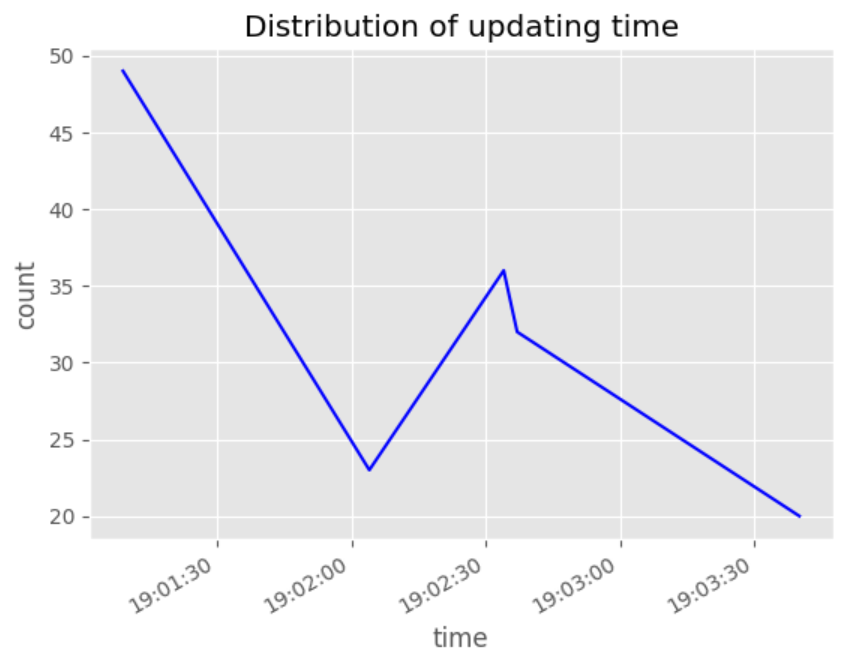
\includegraphics[width=0.75\linewidth]{updatetimes.png}
    \caption{Update times of the ingredients plotted on time axis}
    \label{fig:enter-label}
\end{figure}

\subsection{Questions and answers}
This part will focus on answering some questions about data in 'ingredients' table.
\begin{itemize}
    \item What is top 10 most used types of the ingredients?
    \begin{figure}[H]
        \centering
        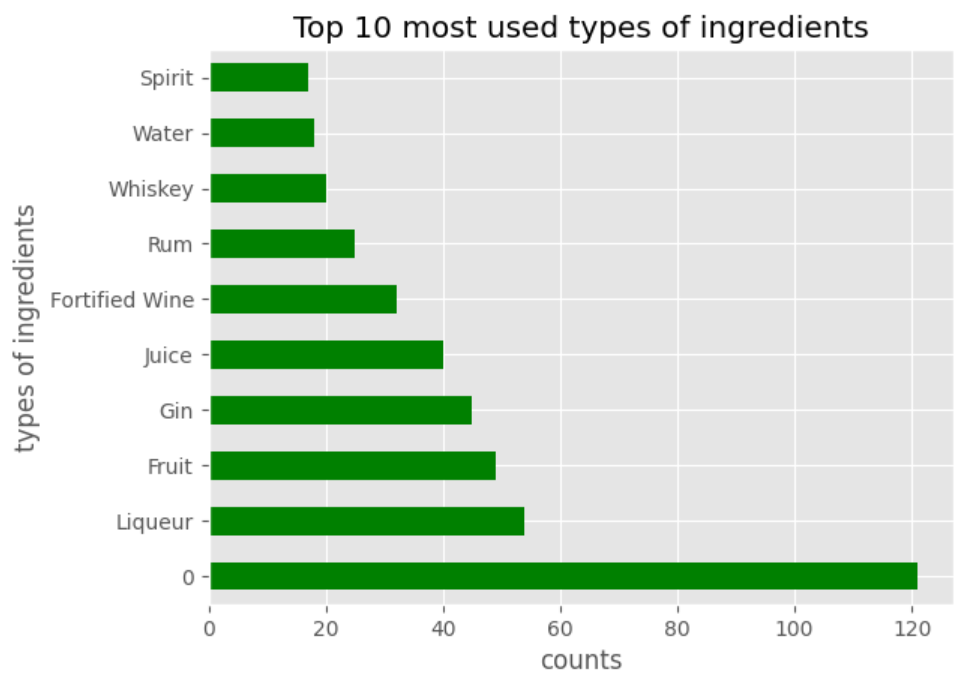
\includegraphics[width=0.9\linewidth]{top10itypes.png}
        \caption{Top 10 most used types of the ingredients}
        \label{fig:enter-label}
    \end{figure}
    Most used ingredient is labeled as a '0'. Knowing that we have replaced every missing values before it means that this category covers ingredients that couldn't have been labeled (ex. water and sugar).

    \item What are the most used ingredients?
    \begin{figure}[H]
        \centering
        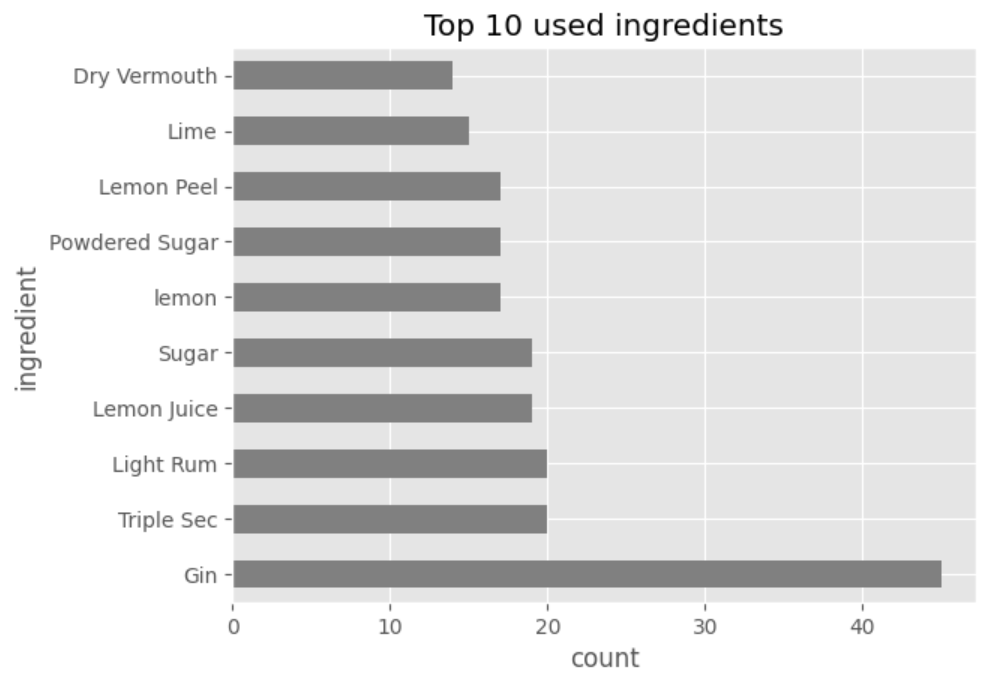
\includegraphics[width=0.9\linewidth]{most used ingr.png}
        \caption{Most used components}
        \label{fig:enter-label}
    \end{figure}
    The most used ingredient is Gin. Next two components in the list are alcohols as well - the main ingredient of the cocktail is the alcohol!

    \item Which ingredients are more populated along all the ingredients: alcoholic or non-alcoholic?
    \begin{figure}[H]
        \centering
        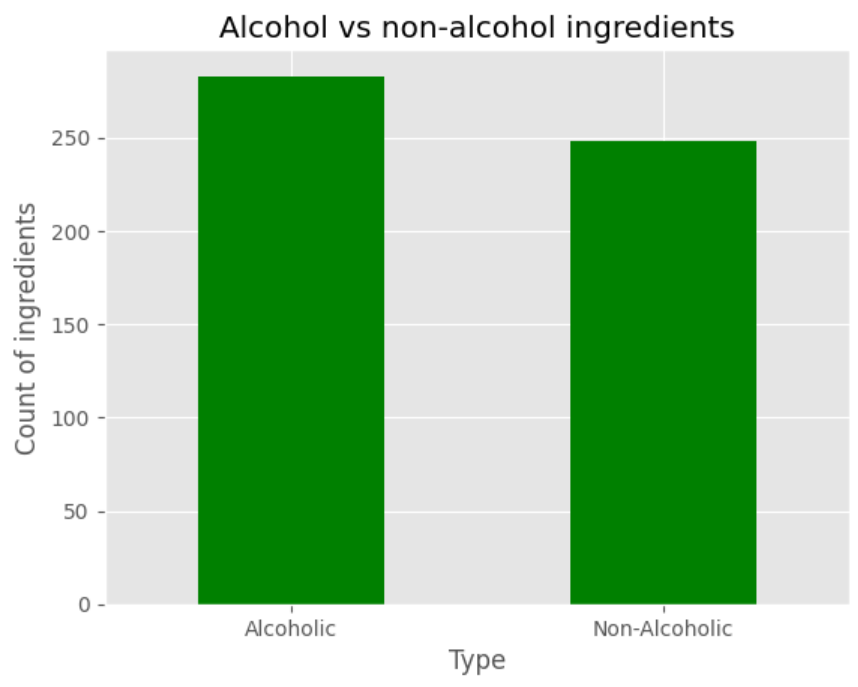
\includegraphics[width=0.8\linewidth]{alcoholicvs.png}
        \caption{Alcoholic vs non-alcoholic ingredients}
        \label{fig:enter-label}
    \end{figure}
    Both types of the ingredients are on similar level with little domination on the alcoholic side. Have in mind that this comparison one cube of an ice is worth as much as one liter of a gin.

    \item What is an average percentage among all of the ingredients?
    Answer: Average percentage per ingredient is: 6.79\%. Every non-alcoholic component of drinks was labeled with 0\%.
\end{itemize}

\section{Analysis of whole dataset}
In this approach we will try to represents each cocktail ingredients as list of indexes. Cocktails will be stored in one DataFrame object and all ingredients will be stored in another DataFrame. We will try to find connections and relations between them. Here is fragment of a code that is responsible for unpacking and storing lists of indexes of ingredients:
\begin{figure}[H]
    \centering
    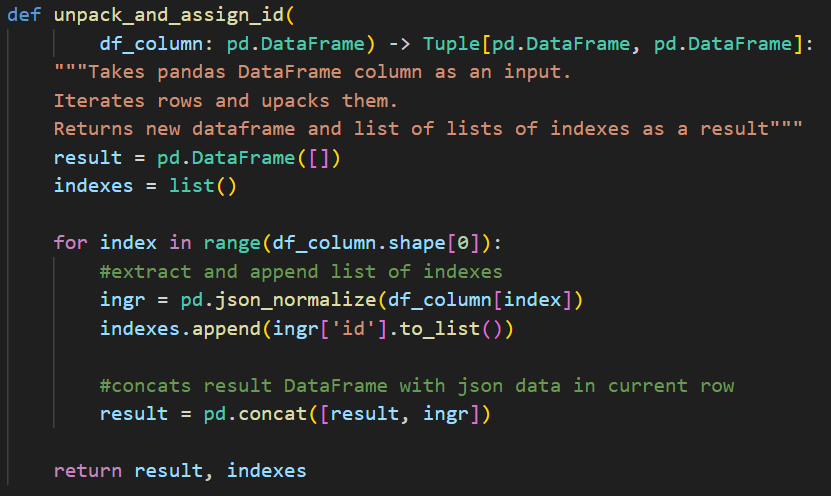
\includegraphics[width=0.9\linewidth]{code_unpacking.png}
    \caption{Fragment of a code representing function which unpacks each list of indexes}
    \label{fig:enter-label}
\end{figure}
Based on previous analyses we drop some of columns:
\begin{itemize}
    \item imageUrl - unnecessary in our analysis
    \item ingredients - we store those in another DataFrame object
    \item tags - missing values
    \item alcoholic - every drink is alcoholic
    \item measure - not normalized
\end{itemize}

\subsection{Questions and answers}
\begin{itemize}
    \item Is there any relationship between instruction length and number of used ingredients?
    \begin{figure}[H]
        \centering
        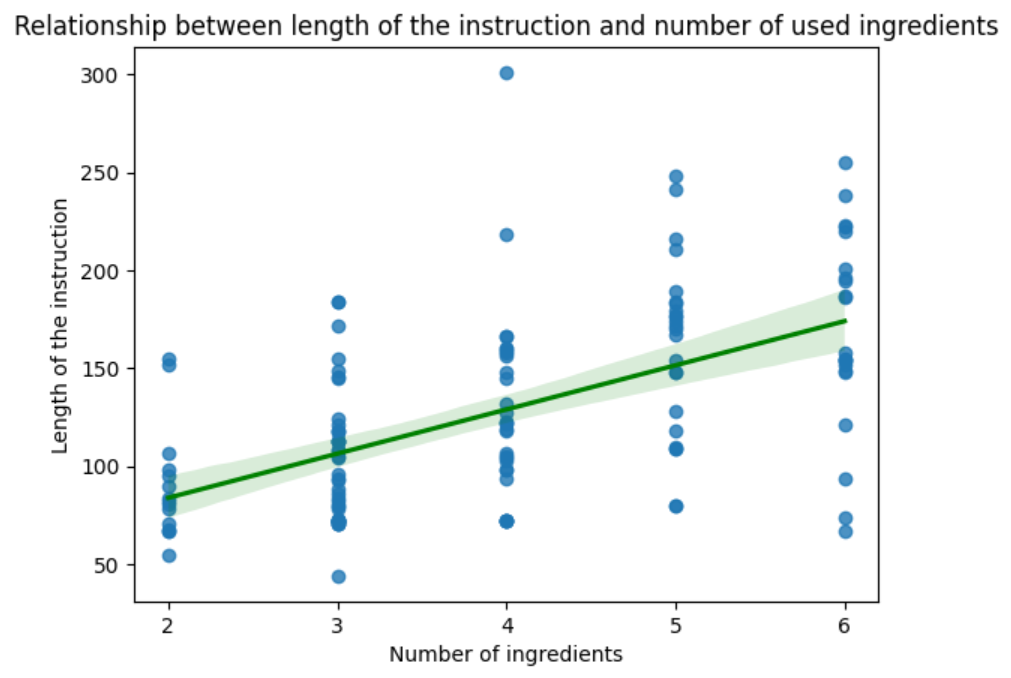
\includegraphics[width=0.75\linewidth]{instructionlen.png}
        \caption{Regression of a instruction length}
        \label{fig:enter-label}
    \end{figure}
    We can clearly see that as number of ingredients grows, length of an instruction is growing. Approximately every additional ingredient adds 20 symbols to length of an instruction.

    \item According to the data, there are around 25 drinks served in an Old-fashioned glass. Which ingredient is the most used in these drinks? To answer this question, we need to filter the DataFrame to include only drinks served in an Old-fashioned glass. Then, for each list of ingredients, we need to find the names of the components and increase the counter for each one. A result shows that most used ingredient in such glass type is powdered sugar which appeared 15 times.
\end{itemize}

\section{Analysis using scikit-learn library}
This sections focuses on analysing our dataset using library that provides a wide range of tools for machine learning, pre-processing, cross-validation, and visualization. We will store data in two tables: drinks and ingredients. This time each drink will have its own record of ingredients listed by name. This will help with vectorizing them.

\subsection{Clustering}
Here we divide our drinks in such a way that objects in the same group (called a cluster) are more similar to each other than to those in other groups. It's a key technique in data mining and machine learning, often used to find hidden patterns or natural groupings in data. Our separation will be based on similarity in used ingredients.

\begin{figure}[H]
    \centering
    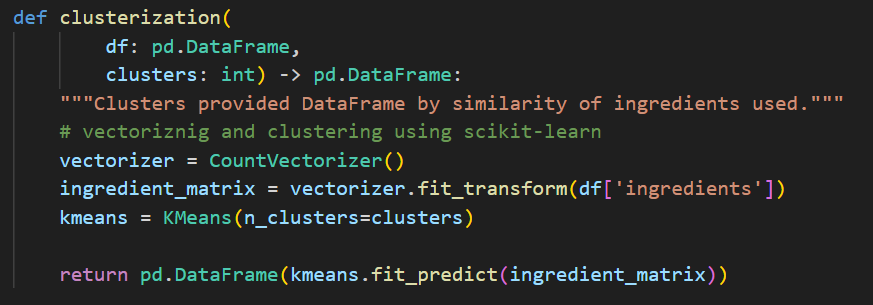
\includegraphics[width=0.9\linewidth]{clusterization.png}
    \caption{Fragment of code representing function used to assign a cluster to each record}
    \label{fig:enter-label}
\end{figure}

Observations shows that dividing data into 3 clusters separates cocktails by ingredients in which indeed drinks have common ingredients. Figure 20 shows that drinks in cluster '1' tends to be made of light rum and some kind of lemon/lime. Cocktails in cluster '0' most likely will consider some kind of sugar (regular, powdered). Drinks in cluster '2' tends to consist of gin and vermouth.

\begin{figure}[H]
    \centering
    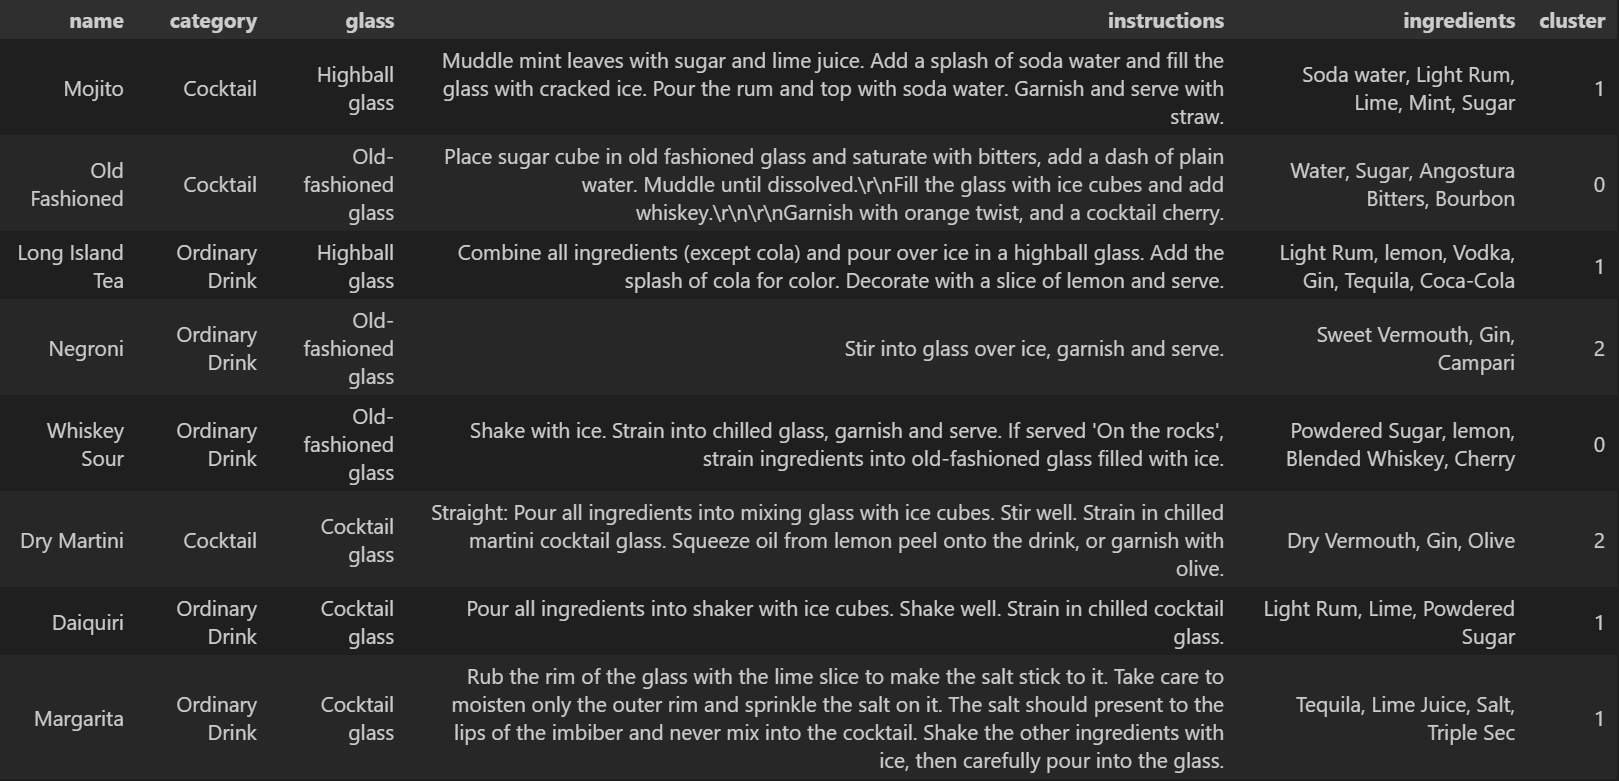
\includegraphics[width=1\linewidth]{clustered head.png}
    \caption{Fragment of a clustered DataFrame}
    \label{fig:enter-label}
\end{figure}

Having each cocktail allotted to a cluster we can transform all to them to a 2D plane which will let us show it on a grid.

\begin{figure}[H]
    \centering
    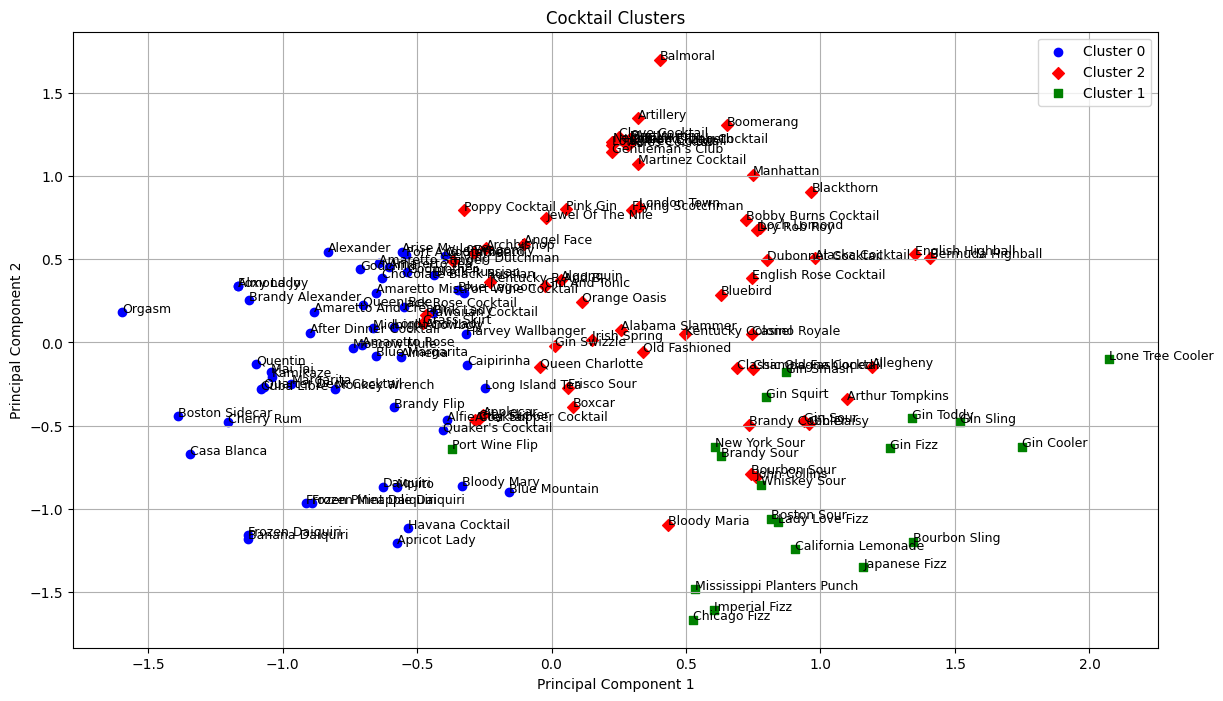
\includegraphics[width=1\linewidth]{plotclusters.png}
    \caption{Clustered data on 2D plane (3 clusters)}
    \label{fig:enter-label}
\end{figure}

\subsection{Cocktail recommendation}
Vectorizing list of ingredients give us plenty other applications. For example for given drink we can find similar one by finding closest point in a space of ingredients. To do such you need to count cosine similarity between given drink and every other, then simply sort list of them. This way you can find most similar (or lest similar) cocktail to the provided one. 

\begin{figure}[H]
    \centering
    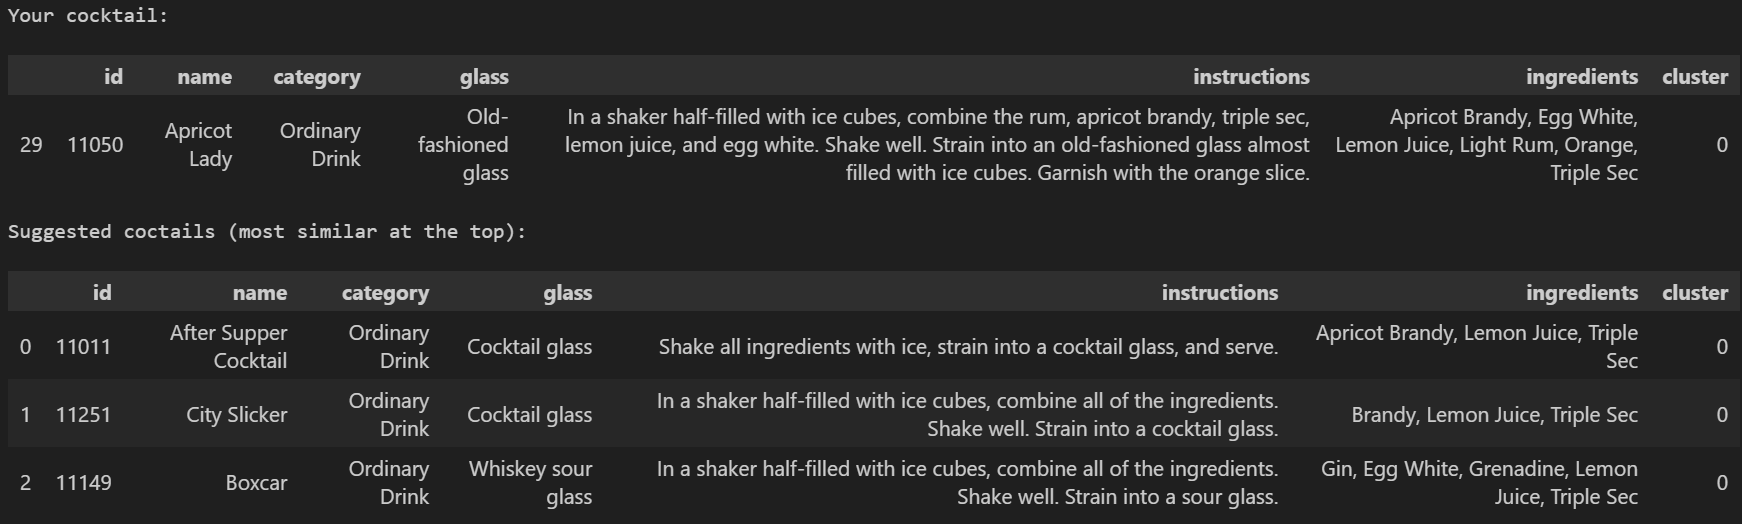
\includegraphics[width=1\linewidth]{recommendedcocktail.png}
    \caption{Results of running recommendation script for 'Apricot Lady'}
    \label{fig:enter-label}
\end{figure}

Observations shows that suggested drinks most often are in a cluster of the provided one. Similarity in ingredients list and the same cluster group proves good clusterization and recommendation.

\section{Results}
The exploratory data analysis of the cocktail dataset, containing 134 drinks and 531 unique ingredients, produced several key findings about the drinks and their ingredient profiles. The data was extensively pre-processed, including handling missing values, excluding uninformative columns, and adjusting for inconsistent IDs and data types. Notable observations include the following:

\subsection{Cocktail Characteristics}
\begin{itemize}
    \item Cocktail instructions varied by glass type; for example, Highball glasses often had longer instructions, possibly reflecting more complex recipes. Categories such as "Cocktail" and "Ordinary Drink" were prevalent, with "Cocktail Glass" being the most commonly used glass type.
    \item Time columns (createdAt, updatedAt) and instruction length were examined for patterns, though no significant trends were uncovered in the creation or update times.
\end{itemize}

\subsection{Ingredient Patterns}
\begin{itemize}
    \item Ingredients such as gin and other alcohol types appeared frequently, reinforcing the central role of alcohol in cocktail composition. Duplicates in the ingredients (e.g., multiple entries for gin) indicated variations in measures and types across cocktails.
    \item Missing values were addressed by assigning zeroes to the missing alcohol percentages, and other incomplete data, such as ingredient types, were excluded from further analyses.
\end{itemize}

\subsection{Clustering and Cocktail Similarity}
\begin{itemize}
    \item A clustering analysis using scikit-learn divided cocktails into three primary clusters based on their ingredient lists. Cluster 1 cocktails often contained light rum and citrus, Cluster 0 cocktails commonly included sugar, and Cluster 2 cocktails were typically made with gin and vermouth.
    \item Vectorization of ingredient lists allowed for cocktail recommendations by identifying the most similar drinks within the same cluster, which was achieved through cosine similarity calculations.
\end{itemize}

\subsection{Additional Insights}
\begin{itemize}
    \item Instruction length showed a linear correlation with the number of ingredients, with each additional ingredient adding approximately 20 characters to the instructions.
    \item Cocktails served in Old-fashioned glasses frequently contained powdered sugar, indicating potential ingredient patterns associated with specific glassware.
\end{itemize}

\section{Conclusions}
The EDA provided a comprehensive understanding of the cocktail dataset and allowed for a successful categorization of drinks based on ingredients and types. The clustering analysis effectively grouped cocktails by ingredient similarity, enabling a structured recommendation system. Several challenges were encountered, including missing values, duplicate entries, and inconsistencies in ingredient measurements. Addressing these issues improved data quality and made clustering and similarity analyses feasible.

\subsection{Perspectives for Further Research}
The insights from this analysis suggest that glass types, ingredient combinations, and instruction lengths can influence the classification of cocktails. Additionally, the recommendation model provides a foundation for further refinement, allowing users to explore similar cocktails based on their ingredient preferences. Future work could involve normalizing measures for more accurate ingredient comparisons and expanding clustering methods to explore additional cocktail attributes.

\subsection{Acknowledgment}
Large language models (LLMs) were used to assist in summarizing the analysis, and all necessary corrections were subsequently made to ensure accuracy and clarity in the report.

\end{document}